\documentclass[12pt,letterpaper]{article}\usepackage[]{graphicx}\usepackage[]{color}
%% maxwidth is the original width if it is less than linewidth
%% otherwise use linewidth (to make sure the graphics do not exceed the margin)
\makeatletter
\def\maxwidth{ %
  \ifdim\Gin@nat@width>\linewidth
    \linewidth
  \else
    \Gin@nat@width
  \fi
}
\makeatother

\definecolor{fgcolor}{rgb}{0.345, 0.345, 0.345}
\newcommand{\hlnum}[1]{\textcolor[rgb]{0.686,0.059,0.569}{#1}}%
\newcommand{\hlstr}[1]{\textcolor[rgb]{0.192,0.494,0.8}{#1}}%
\newcommand{\hlcom}[1]{\textcolor[rgb]{0.678,0.584,0.686}{\textit{#1}}}%
\newcommand{\hlopt}[1]{\textcolor[rgb]{0,0,0}{#1}}%
\newcommand{\hlstd}[1]{\textcolor[rgb]{0.345,0.345,0.345}{#1}}%
\newcommand{\hlkwa}[1]{\textcolor[rgb]{0.161,0.373,0.58}{\textbf{#1}}}%
\newcommand{\hlkwb}[1]{\textcolor[rgb]{0.69,0.353,0.396}{#1}}%
\newcommand{\hlkwc}[1]{\textcolor[rgb]{0.333,0.667,0.333}{#1}}%
\newcommand{\hlkwd}[1]{\textcolor[rgb]{0.737,0.353,0.396}{\textbf{#1}}}%

\usepackage{framed}
\makeatletter
\newenvironment{kframe}{%
 \def\at@end@of@kframe{}%
 \ifinner\ifhmode%
  \def\at@end@of@kframe{\end{minipage}}%
  \begin{minipage}{\columnwidth}%
 \fi\fi%
 \def\FrameCommand##1{\hskip\@totalleftmargin \hskip-\fboxsep
 \colorbox{shadecolor}{##1}\hskip-\fboxsep
     % There is no \\@totalrightmargin, so:
     \hskip-\linewidth \hskip-\@totalleftmargin \hskip\columnwidth}%
 \MakeFramed {\advance\hsize-\width
   \@totalleftmargin\z@ \linewidth\hsize
   \@setminipage}}%
 {\par\unskip\endMakeFramed%
 \at@end@of@kframe}
\makeatother

\definecolor{shadecolor}{rgb}{.97, .97, .97}
\definecolor{messagecolor}{rgb}{0, 0, 0}
\definecolor{warningcolor}{rgb}{1, 0, 1}
\definecolor{errorcolor}{rgb}{1, 0, 0}
\newenvironment{knitrout}{}{} % an empty environment to be redefined in TeX

\usepackage{alltt}
 \usepackage[left=2cm,right=2cm,top=2cm,bottom=2cm]{geometry}
\usepackage[ansinew]{inputenc}
\usepackage[spanish]{babel}
\usepackage{amsmath}
\usepackage{amsfonts}
\usepackage{amssymb}
\usepackage{dsfont}
\usepackage{multicol} 
\usepackage{subfigure}
\usepackage{graphicx}
\usepackage{float} 
\usepackage{verbatim} 
\usepackage[left=2cm,right=2cm,top=2cm,bottom=2cm]{geometry}
\usepackage{fancyhdr}
\pagestyle{fancy} 
\fancyhead[LO]{\leftmark}
\usepackage{caption}
\newtheorem{definicion}{Definci\'on}
\IfFileExists{upquote.sty}{\usepackage{upquote}}{}
\begin{document}

\begin{titlepage}
\setlength{\unitlength}{1 cm} %Especificar unidad de trabajo


\begin{center}
\textbf{{\large UNIVERSIDAD DE EL SALVADOR}\\
{\large FACULTAD MULTIDISCIPLINARIA DE OCCIDENTE}\\
{\large DEPARTAMENTO DE MATEM\'ATICA}}\\[0.50 cm]

\begin{picture}(18,4)
 \put(7,0){
\includegraphics[width=4cm]{minerva.jpg}}
\end{picture}
\\[0.25 cm]

\textbf{{\large Licenciatura en Estad\'istica}\\[1.25cm]
{\large Control Estadistico del Paquete R }\\[2 cm]
%\setlength{\unitlength}{1 cm}
{\large  \textbf{''UNIDAD TRES"}}\\
{\large  \textbf{Pr\'actica 15 - Distribuciones de probabilidad continuas.}}\\[3 cm]
{\large Alumna:}\\
{\large Martha Yoana Medina S\'anchez}\\[2cm]
{\large Fecha de elaboraci\'on}\\
Santa Ana - \today }
\end{center}
\end{titlepage}

\newtheorem{teorema}{Teorema}
\newtheorem{prop}{Proposici\'on}[section]

\lhead{UNIDAD TRES}
\chead{PR\'ACTICA 15}
\lfoot{LICENCIATURA EN ESTAD\'ISTICA}
\cfoot{UESOCC}
\rfoot{\thepage}
%\pagestyle{fancy} 

\setcounter{page}{1}
\newpage

\begin{center}
  \textbf {1. DISTRIBUCIONES CONTINUAS.} 
\end{center}
\begin{description}
  \item \textbf{a) Distribuc\'ion uniforme.}
\end{description}

\begin{itemize}
  \item \textbf{Par\'ametros.}
  \begin{center}
x = valor cualquiera\\ 
p = probabilidad\\
n = tama\~no de la muestra\\ 
min = valor m\'inimo\\ 
max = valor m\'aximo\\
\end{center}
\item \textbf{Sintaxis de la funci\'on utilizada en R}
\begin{enumerate}
  \item punif(x, min, max, lower.tail = TRUE, log.p = FALSE)
  \item qunif(p, min, max, lower.tail = TRUE, log.p = FALSE) 
  \item runif(n, min, max) 
\end{enumerate}
\end{itemize}

\begin{description}
  \item \textbf{b) Distribuc\'ion Normal.}\\
\end{description}

\begin{itemize}
  \item \textbf{Par\'ametros.}
  \begin{center}
x = valor cualquiera\\ 
p = probabilidad\\ 
mean = media\\ 
sd = desviación t\'ipica\\ 
n = tama\~no de la muestra\\ 
\end{center}
\item \textbf{Sintaxis de la funci\'on utilizada en R}
\begin{enumerate}
  \item pnorm(x, mean, sd, lower.tail = TRUE, log.p = FALSE) 
  \item qnorm(p, mean, sd, lower.tail = TRUE, log.p = FALSE) 
  \item rnorm(n, mean, sd)  
\end{enumerate}
\end{itemize}

\begin{description}
  \item \textbf{c) Distribuc\'ion T-Student.}
\end{description}
\begin{itemize}
  \item \textbf{Par\'ametros.}
  \begin{center}
x = valor cualquiera\\ 
p = probabilidad\\
df = grados de libertad\\  
\end{center}
\item \textbf{Sintaxis de la funci\'on utilizada en R}
\begin{enumerate}
  \item pt(x, df, lower.tail = TRUE, log.p = FALSE)
  \item pt(x, df, lower.tail = TRUE, log.p = FALSE) 
  \item rt(n, df)   
\end{enumerate}
\end{itemize}

\begin{description}
  \item \textbf{d) Distribuc\'ion Chi-cuadrado.}
\end{description}
\begin{itemize}
  \item \textbf{Par\'ametros.}
  \begin{center}
x = valor cualquiera\\ 
df = grados de libertad\\ 
p = probabilidad\\  
\end{center}
\item \textbf{Sintaxis de la funci\'on utilizada en R}
\begin{enumerate}
  \item pchisq(x, df, lower.tail = TRUE, log.p = FALSE)
  \item qchisq(p, df, lower.tail = TRUE, log.p = FALSE)
  \item rchisq(n, df,)    
\end{enumerate}
\end{itemize}

\begin{description}
  \item \textbf{d) Distribuc\'ion F de Snedecor.}
\end{description}
\begin{itemize}
  \item \textbf{Par\'ametros.}
  \begin{center}
x,q = vector cuantiles\\ 
df1 = grados de libertad en el numerador\\ 
df2 = grados de libertad en el denominador\\ 
p = vector probabilidad\\
\end{center}
\item \textbf{Sintaxis de la funci\'on utilizada en R}
\begin{enumerate}
  \item pf(q, df1, df2, ncp, lower.tail = TRUE, log.p = FALSE)
  \item qf(p, df1, df2, ncp, lower.tail=TRUE, log.p = FALSE) 
  \item rf(n, df1, df2, ncp) 
\end{enumerate}
\end{itemize}

\begin{description}
  \item \textbf{d) Distribuc\'ion Exponencial.}
\end{description}
\begin{itemize}
  \item \textbf{Par\'ametros.}
  \begin{center}
x,q = vector cuantiles\\ 
rate = raz\'on = 1/E[X]\\
p = vector probabilidad \\
lower.tail = T \\
\end{center}
\item \textbf{Sintaxis de la funci\'on utilizada en R}
\begin{enumerate}
  \item pexp(q, rate = 1, lower.tail = TRUE, log.p = FALSE)
  \item qexp(p, rate = 1, lower.tail = TRUE, log.p = FALSE)
  \item rexp(n, rate = 1)  
\end{enumerate}
\end{itemize}

\begin{center}
\textbf{2.  C\'ALCULO DE PROBABILIDADES.}
\end{center}
\begin{itemize}
  \item \textbf{Ejemplo 1:}
\end{itemize}

Una persona informal hace esperar a su pareja aleatoriamente entre 0 y 90 minutos. Harto de esta situaci\'on, la persona que sufre la espera se plantea un ultim\'atum; s\'i al d\'ia siguiente su pareja tarda menos de 15 minutos mantiene la relaci\'on, s\'i la espera est\'a entre 15 y 55 minutos, decide en la siguiente cita con los mismos criterios, mientras que si tarda m\'as de 55 minutos la relaci\'on termina en ese momento.

\begin{description}
  \item a) Calcule la probabilidad de que la relaci'on contin\'ue hasta la siguiente cita. 
\begin{knitrout}
\definecolor{shadecolor}{rgb}{0.969, 0.969, 0.969}\color{fgcolor}\begin{kframe}
\begin{alltt}
\hlstd{x} \hlkwb{<-} \hlnum{55}\hlstd{; a}\hlkwb{=}\hlnum{0}\hlstd{; b} \hlkwb{<-} \hlnum{90}

\hlcom{# usando la funcion propia de R }

\hlkwd{punif}\hlstd{(x,} \hlkwc{min}\hlstd{=a,} \hlkwc{max}\hlstd{=b,} \hlkwc{lower.tail}\hlstd{=}\hlnum{TRUE}\hlstd{)}
\end{alltt}
\begin{verbatim}
## [1] 0.6111111
\end{verbatim}
\end{kframe}
\end{knitrout}
\end{description}

\begin{description}
  \item b) Calcule la probabilidad de que la relaci\'on termine en la segunda cita.\\
  
Suponiendo que el tiempo de espera en una cita es independiente respecto de otras citas, se calcula la probabilidad P(15$<$X$<$55) = P(X$<$55) - P(X$<$=15) = 0.6111 - 0.1666 = 0.4445,
\begin{knitrout}
\definecolor{shadecolor}{rgb}{0.969, 0.969, 0.969}\color{fgcolor}\begin{kframe}
\begin{alltt}
\hlstd{F55}\hlkwb{=}\hlkwd{punif}\hlstd{(}\hlnum{55}\hlstd{,} \hlkwc{min}\hlstd{=a,} \hlkwc{max}\hlstd{=b,} \hlkwc{lower.tail}\hlstd{=}\hlnum{TRUE}\hlstd{)}
\hlstd{F15}\hlkwb{=}\hlkwd{punif}\hlstd{(}\hlnum{15}\hlstd{,} \hlkwc{min}\hlstd{=a,} \hlkwc{max}\hlstd{=b,} \hlkwc{lower.tail}\hlstd{=}\hlnum{TRUE}\hlstd{)}
\hlstd{F55}\hlopt{-}\hlstd{F15}
\end{alltt}
\begin{verbatim}
## [1] 0.4444444
\end{verbatim}
\end{kframe}
\end{knitrout}
\end{description}
que es la probabilidad de que aplace la decisi\'on para la segunda cita y, en la segunda cita, la probabilidad de que lo deje definitivamente es P(X$>$55) = 0.3888,
\begin{knitrout}
\definecolor{shadecolor}{rgb}{0.969, 0.969, 0.969}\color{fgcolor}\begin{kframe}
\begin{alltt}
\hlstd{F55}\hlkwb{=}\hlkwd{punif}\hlstd{(}\hlnum{55}\hlstd{,} \hlkwc{min}\hlstd{=a,} \hlkwc{max}\hlstd{=b,} \hlkwc{lower.tail}\hlstd{=}\hlnum{TRUE}\hlstd{);F55}
\end{alltt}
\begin{verbatim}
## [1] 0.6111111
\end{verbatim}
\end{kframe}
\end{knitrout}
luego multiplicando ambas probabilidades se obtiene el valor pedido 0.1728.
\begin{knitrout}
\definecolor{shadecolor}{rgb}{0.969, 0.969, 0.969}\color{fgcolor}\begin{kframe}
\begin{alltt}
\hlstd{(}\hlnum{1}\hlopt{-}\hlstd{F55)}\hlopt{*}\hlstd{( F55}\hlopt{-}\hlstd{F15)}
\end{alltt}
\begin{verbatim}
## [1] 0.1728395
\end{verbatim}
\end{kframe}
\end{knitrout}

\begin{itemize}
  \item \textbf{Ejemplo 2:}
\end{itemize}

Una empresa est\'a buscando personal para su departamento de mercadeo. El perfil solicitado es el de sujetos extrovertidos y creativos. Se han presentado 50 candidatos y la empresa ha establecido como criterio de selecci\'on que los candidatos superen el percentil 80 en creatividad y extroversi\'on. Sabiendo que la variable extroversi\'on (X) se distribuye seg\'un una Normal de media 5 y desviaci\'on t\'ipica 1, que la variable creatividad (Y) sigue una t-Student de 10 grados de libertad y que las puntuaciones de creatividad y extroversi\'on son independientes: 
\begin{description}
  \item a) \¿Cu\'antos candidatos ser\'an seleccionados?
  
Al ser X e Y independientes, la probabilidad:

P(X$>$=P80nY$>$=P80)=P(X$>$=P80)P(Y$>$=P80)=(0.20)(0.20)=0.04\\  
Como se han presentado 50 aspirantes, ser\'an seleccionadas (50)(0.04)=2 personas.
\end{description}

\begin{description}
  \item b) \¿Qu\'e puntuaciones debe superar un aspirante en creatividad y extroversi\'on para ser admitido?
  
Seg\'un el criterio de selecci\'on se debe superar el percentil 80, en ambas variables, para ser admitido. Se calcular\'a pues el percentil 80 de la variable X e Y,utilizando los cuantiles-normales para la variable X: 
\begin{knitrout}
\definecolor{shadecolor}{rgb}{0.969, 0.969, 0.969}\color{fgcolor}\begin{kframe}
\begin{alltt}
\hlcom{# y los cuantiles-normales para la variable X:}

\hlstd{p} \hlkwb{<-} \hlkwd{c}\hlstd{(}\hlnum{0.80}\hlstd{); media}\hlkwb{=}\hlnum{5}\hlstd{; d.t}\hlkwb{=}\hlnum{1}
\hlkwd{qnorm}\hlstd{(p,} \hlkwc{mean}\hlstd{=media,} \hlkwc{sd}\hlstd{=d.t,} \hlkwc{lower.tail}\hlstd{=}\hlnum{TRUE}\hlstd{)}
\end{alltt}
\begin{verbatim}
## [1] 5.841621
\end{verbatim}
\end{kframe}
\end{knitrout}

\begin{knitrout}
\definecolor{shadecolor}{rgb}{0.969, 0.969, 0.969}\color{fgcolor}\begin{kframe}
\begin{alltt}
\hlcom{#y los cuantiles-t para la variable Y:}

\hlstd{p} \hlkwb{<-} \hlkwd{c}\hlstd{(}\hlnum{0.80}\hlstd{); g.l} \hlkwb{<-} \hlnum{10}
\hlkwd{qt}\hlstd{(p,} \hlkwc{df}\hlstd{=g.l,} \hlkwc{lower.tail}\hlstd{=}\hlnum{TRUE}\hlstd{)}
\end{alltt}
\begin{verbatim}
## [1] 0.8790578
\end{verbatim}
\end{kframe}
\end{knitrout}
\end{description}

\begin{description}
  \item c) Si se extraen al azar 16 candidatos, \¿cu\'al es la probabilidad de que su media aritm\'etica en extroversi\'on sea mayor que 4.5? 
Se sabe que al extraer una muestra de una poblaci\'on normal de tama\~no n, lamedia muestral, sigue otra distribuci\'on normal de media igual que la poblacional y desviaci\'on t\'ipica sigma/sqrt(n).\\

Como se desea calcular P(media$>$=4.5):
\begin{knitrout}
\definecolor{shadecolor}{rgb}{0.969, 0.969, 0.969}\color{fgcolor}\begin{kframe}
\begin{alltt}
\hlstd{n} \hlkwb{<-} \hlnum{16}\hlstd{; x} \hlkwb{<-} \hlnum{4.5}\hlstd{; mu}\hlkwb{=}\hlnum{5}\hlstd{; sigma}\hlkwb{=}\hlnum{1}\hlstd{; d.t}\hlkwb{=}\hlstd{sigma}\hlopt{/}\hlkwd{sqrt}\hlstd{(n)}
\hlkwd{pnorm}\hlstd{(x,} \hlkwc{mean}\hlstd{=mu,} \hlkwc{sd}\hlstd{=d.t,} \hlkwc{lower.tail}\hlstd{=}\hlnum{FALSE}\hlstd{)}
\end{alltt}
\begin{verbatim}
## [1] 0.9772499
\end{verbatim}
\end{kframe}
\end{knitrout}
\end{description}

\begin{itemize}
  \item \textbf{Ejemplo 3:}
\end{itemize}
La duraci\'on media de un modelo de marcapasos es de 7 a\~nos. 
\begin{description}
  \item a) \¿Cu\'al es la probabilidad de que dure al menos 5 a\~nos? \¿y menos de 3 a\~nos?
  
Suponiendo que la variable X="tiempo de funcionamiento del marcapasos" sigue una distribuci\'on exponencial.

La probabilidad P(X$>$=5) se obtiene as\'i:
\begin{knitrout}
\definecolor{shadecolor}{rgb}{0.969, 0.969, 0.969}\color{fgcolor}\begin{kframe}
\begin{alltt}
\hlstd{x} \hlkwb{<-} \hlnum{5}\hlstd{; teta}\hlkwb{=}\hlnum{7}
\hlkwd{pexp}\hlstd{(x,} \hlkwc{rate}\hlstd{=}\hlnum{1}\hlopt{/}\hlstd{teta,} \hlkwc{lower.tail}\hlstd{=}\hlnum{FALSE}\hlstd{)}
\end{alltt}
\begin{verbatim}
## [1] 0.4895417
\end{verbatim}
\end{kframe}
\end{knitrout}

y de igual forma  P(X$<$3): 
\begin{knitrout}
\definecolor{shadecolor}{rgb}{0.969, 0.969, 0.969}\color{fgcolor}\begin{kframe}
\begin{alltt}
\hlstd{x} \hlkwb{<-} \hlnum{3}\hlstd{; teta}\hlkwb{=}\hlnum{7}
\hlkwd{pexp}\hlstd{(x,} \hlkwc{rate}\hlstd{=}\hlnum{1}\hlopt{/}\hlstd{teta,} \hlkwc{lower.tail}\hlstd{=}\hlnum{TRUE}\hlstd{)}
\end{alltt}
\begin{verbatim}
## [1] 0.3485609
\end{verbatim}
\end{kframe}
\end{knitrout}


  \item b) Si han transcurrido ya 4 a\~nos desde su implantaci\'on, \¿cu\'al es la probabilidad de que dure otros 4? Nos piden P(X$>$=8/X$>$=4)
  
Teniendo en cuenta que la funci\'on de distribuci\'on es la \'unica distribuci\'on continua no tiene memoria resulta que P(X$>$=8/X$>$=4)=P(X$>$=4)=0.5647182
\begin{knitrout}
\definecolor{shadecolor}{rgb}{0.969, 0.969, 0.969}\color{fgcolor}\begin{kframe}
\begin{alltt}
\hlkwd{pexp}\hlstd{(}\hlnum{4}\hlstd{,} \hlkwc{rate}\hlstd{=}\hlnum{1}\hlopt{/}\hlstd{teta,} \hlkwc{lower.tail}\hlstd{=}\hlnum{FALSE}\hlstd{)}
\end{alltt}
\begin{verbatim}
## [1] 0.5647181
\end{verbatim}
\end{kframe}
\end{knitrout}

\item c) \¿Cu\'anto tiempo deber\'ia funcionar un marcapasos para estar entre el 10\% de los que m\'as duran?

Hay que calcular el percentil 90:
\begin{knitrout}
\definecolor{shadecolor}{rgb}{0.969, 0.969, 0.969}\color{fgcolor}\begin{kframe}
\begin{alltt}
\hlstd{p} \hlkwb{<-} \hlnum{0.9}\hlstd{; teta} \hlkwb{<-} \hlnum{7}
\hlkwd{qexp}\hlstd{(p,} \hlkwc{rate}\hlstd{=}\hlnum{1}\hlopt{/}\hlstd{teta,} \hlkwc{lower.tail}\hlstd{=}\hlnum{TRUE}\hlstd{)}
\end{alltt}
\begin{verbatim}
## [1] 16.1181
\end{verbatim}
\begin{alltt}
\hlcom{#resultando 16.12 a\textbackslash{}~nos. }
\end{alltt}
\end{kframe}
\end{knitrout}

\item d) Calcular el valor que deben tener a y b para que P(X$<$a)=0.5 PX a 0.5 y P(X$>$b)=0.32

De forma an\'aloga al apartado anterior, en el primer caso habr\'ia que calcular la mediana (percentil 50), a = 4.852,
\begin{knitrout}
\definecolor{shadecolor}{rgb}{0.969, 0.969, 0.969}\color{fgcolor}\begin{kframe}
\begin{alltt}
\hlkwd{qexp}\hlstd{(}\hlnum{0.5}\hlstd{,} \hlkwc{rate}\hlstd{=}\hlnum{1}\hlopt{/}\hlstd{teta,} \hlkwc{lower.tail}\hlstd{=}\hlnum{TRUE}\hlstd{)}
\end{alltt}
\begin{verbatim}
## [1] 4.85203
\end{verbatim}
\end{kframe}
\end{knitrout}
\begin{knitrout}
\definecolor{shadecolor}{rgb}{0.969, 0.969, 0.969}\color{fgcolor}\begin{kframe}
\begin{alltt}
\hlcom{# y en el segundo caso, el percentil 68, b = 7.97}

\hlkwd{qexp}\hlstd{(}\hlnum{0.68}\hlstd{,} \hlkwc{rate}\hlstd{=}\hlnum{1}\hlopt{/}\hlstd{teta,} \hlkwc{lower.tail}\hlstd{=}\hlnum{TRUE}\hlstd{)}
\end{alltt}
\begin{verbatim}
## [1] 7.97604
\end{verbatim}
\end{kframe}
\end{knitrout}
\begin{knitrout}
\definecolor{shadecolor}{rgb}{0.969, 0.969, 0.969}\color{fgcolor}\begin{kframe}
\begin{alltt}
\hlcom{# o de esta otra manera}

\hlkwd{qexp}\hlstd{(}\hlnum{0.32}\hlstd{,} \hlkwc{rate}\hlstd{=}\hlnum{1}\hlopt{/}\hlstd{teta,} \hlkwc{lower.tail}\hlstd{=}\hlnum{FALSE}\hlstd{)}
\end{alltt}
\begin{verbatim}
## [1] 7.97604
\end{verbatim}
\end{kframe}
\end{knitrout}
\end{description}

\newpage

\begin{center}
\textbf{3.  GENERACI\'ON DE MUESTRAS ALEATORIAS DE LAS DISTRIBUCIONES.} 
\end{center}

\begin{itemize}
  \item \textbf{Ejemplo 1:}
\end{itemize}
Generar 100 n\'umeros aleatorios de una distribuci\'on Uniforme en [-2, 4]
\begin{knitrout}
\definecolor{shadecolor}{rgb}{0.969, 0.969, 0.969}\color{fgcolor}\begin{kframe}
\begin{alltt}
\hlcom{# Definir los par\textbackslash{}'ametros apropiados}
\hlstd{min} \hlkwb{<-} \hlopt{-}\hlnum{2}\hlstd{; max} \hlkwb{<-} \hlnum{4}

\hlcom{# generar 100 n\textbackslash{}'umeros aleatorios de la distribuci\textbackslash{}'on }
\hlstd{x} \hlkwb{=} \hlkwd{runif}\hlstd{(}\hlnum{100}\hlstd{, min, max); x}
\end{alltt}
\begin{verbatim}
##   [1]  1.93536984  0.48794002  3.16088643 -1.98006110 -0.12364830
##   [6]  0.36497971 -0.36620827  1.10462600 -0.53854729 -0.31606691
##  [11]  2.44961394  2.54016676 -0.19798646 -1.11801856  2.38775964
##  [16] -0.37759314 -0.87407659  0.98529517 -0.62860891  3.24161901
##  [21] -1.42665437  1.55476034  1.72200572  1.69594416  1.18840346
##  [26] -0.58345596  0.83782765  2.08484564 -0.58484657  1.40401472
##  [31]  0.73504179  3.68171236  0.36219574  1.14706969 -0.45818063
##  [36]  1.02862697 -0.42317659  1.13967025  1.70840789  0.81792576
##  [41]  3.00270698 -1.28102504  3.75752606  3.21890690 -1.23027636
##  [46]  3.63390102  3.88954588  0.62900457  1.01934674  1.53893361
##  [51]  1.82253061 -0.32833368  2.30456683 -0.37287721 -1.35619000
##  [56]  3.66513973  0.28910594 -0.13040638 -1.22198929  2.41731965
##  [61] -1.26216745 -0.31702129  0.71153323  0.47789773  3.54506094
##  [66]  1.40899352  3.49292276  3.06245976  2.84756282  3.55149454
##  [71] -1.68034053  3.10631353  2.64125899 -0.72169913  3.28513325
##  [76] -0.72832528  1.42706489  2.56976939  0.96727307 -0.54222676
##  [81]  0.49741977  0.84228006  3.84567078  3.79354362 -1.88182253
##  [86]  2.71978739 -1.04190263  1.34329914  0.47078387  0.02234774
##  [91] -1.41659411 -0.79560201  2.56052075  0.64063966 -1.59104959
##  [96]  2.12727118  2.12708346  0.64837956  3.33574958  0.59836524
\end{verbatim}
\begin{alltt}
\hlcom{# Histograma para la nuestra aleatoria de tama\textbackslash{}~no 100 }
\hlkwd{hist}\hlstd{(x,} \hlkwc{main}\hlstd{=}\hlstr{"X ~ Uniforme(min=-2, max=4"}\hlstd{,} \hlkwc{xlab}\hlstd{=}\hlstr{"X"}\hlstd{,}
     \hlkwc{ylab}\hlstd{=}\hlstr{"densidad de probabilidad"}\hlstd{,} \hlkwc{probability}\hlstd{=}\hlnum{TRUE}\hlstd{,} \hlkwc{col}\hlstd{=}\hlstr{"green"}\hlstd{)}

\hlcom{# Graficar la funci\textbackslash{}'on de densidad, use la funci\textbackslash{}'on curve() para variable continua }
\hlkwd{curve}\hlstd{(}\hlkwd{dunif}\hlstd{(x, min, max),} \hlkwc{col}\hlstd{=}\hlstr{"blue"}\hlstd{,} \hlkwc{add}\hlstd{=}\hlnum{TRUE}\hlstd{)}
\end{alltt}
\end{kframe}
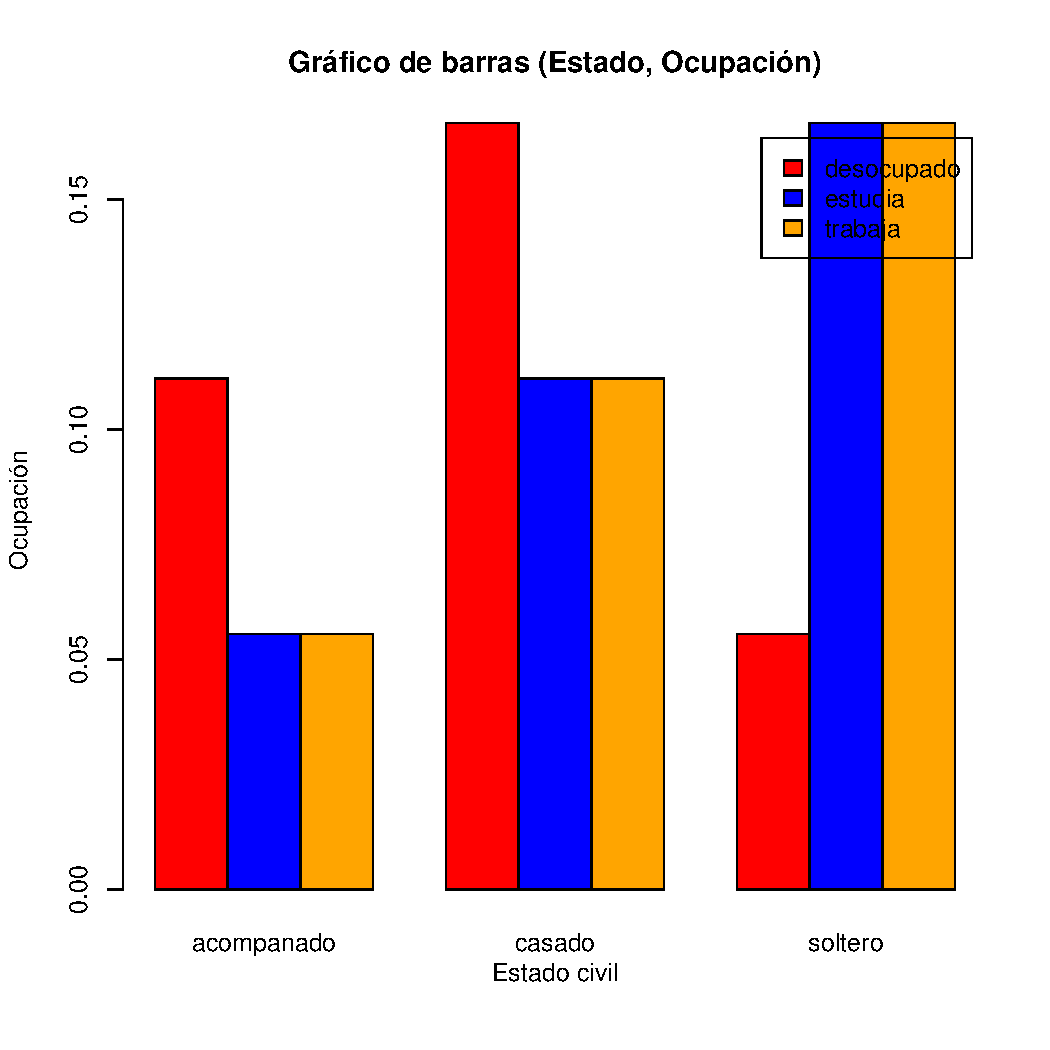
\includegraphics[width=\maxwidth]{figure/unnamed-chunk-15-1} 

\end{knitrout}

\begin{itemize}
  \item \textbf{Ejemplo 2:}
\end{itemize}
Supongamos que tenemos una muestra de tama\~no n=200 perteneciente a una poblaci\'on normal N(10,2) con media igual a 10 y con una desviaci\'on estandar igual a 2:
\begin{knitrout}
\definecolor{shadecolor}{rgb}{0.969, 0.969, 0.969}\color{fgcolor}\begin{kframe}
\begin{alltt}
\hlcom{# genera los valores aleatorios de la distribuci\textbackslash{}'on }
\hlstd{x.norm} \hlkwb{<-} \hlkwd{rnorm}\hlstd{(}\hlkwc{n}\hlstd{=}\hlnum{200}\hlstd{,}\hlkwc{mean}\hlstd{=}\hlnum{10}\hlstd{,} \hlkwc{sd}\hlstd{=}\hlnum{2}\hlstd{)}

\hlcom{# Podemos obtener un histograma usando la funci\textbackslash{}'on hist() }
\hlkwd{hist}\hlstd{(x.norm,} \hlkwc{breaks} \hlstd{=} \hlstr{"Sturges"}\hlstd{,} \hlkwc{freq} \hlstd{=} \hlnum{TRUE}\hlstd{,} \hlkwc{probability} \hlstd{=} \hlnum{FALSE}\hlstd{,}
     \hlkwc{include.lowest} \hlstd{=} \hlnum{TRUE}\hlstd{,} \hlkwc{right} \hlstd{=} \hlnum{TRUE}\hlstd{,} \hlkwc{density} \hlstd{=} \hlkwa{NULL}\hlstd{,}
\hlkwc{angle} \hlstd{=} \hlnum{45}\hlstd{,} \hlkwc{col} \hlstd{=} \hlstr{"steelblue1"}\hlstd{,} \hlkwc{border} \hlstd{=} \hlkwa{NULL}\hlstd{,}
\hlkwc{main} \hlstd{=} \hlstr{"Histograma de datos observados"}\hlstd{,} \hlkwc{axes} \hlstd{=} \hlnum{TRUE}\hlstd{,}
\hlkwc{plot} \hlstd{=} \hlnum{TRUE}\hlstd{,} \hlkwc{labels} \hlstd{=} \hlnum{FALSE}\hlstd{)}
\end{alltt}
\end{kframe}
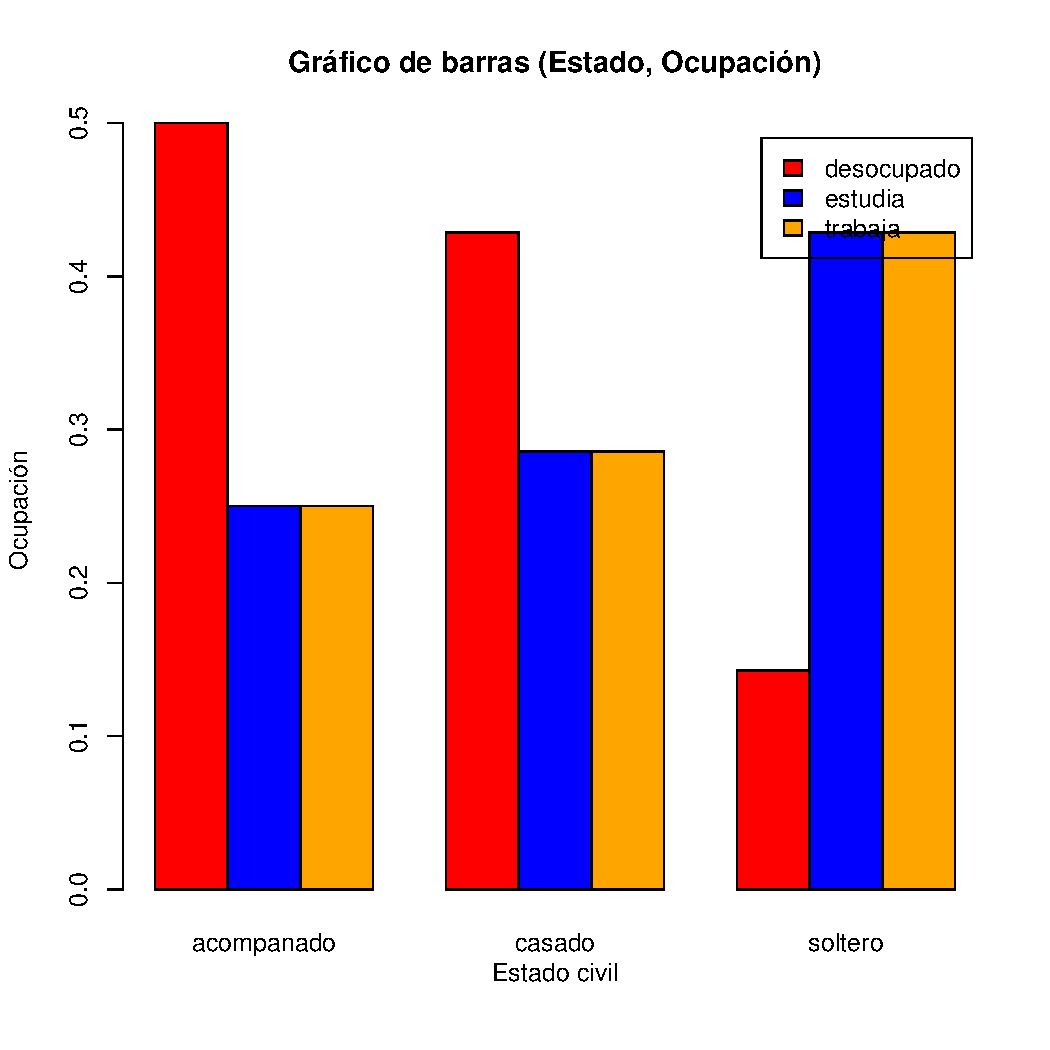
\includegraphics[width=\maxwidth]{figure/unnamed-chunk-16-1} 
\begin{kframe}\begin{alltt}
\hlcom{# Podemos estimar la densidad de frecuencia usando la funci\textbackslash{}'on }
\hlcom{# density() y plot() para dibujar su }
\hlstr{"gráfica"}
\end{alltt}
\begin{verbatim}
## [1] "gráfica"
\end{verbatim}
\begin{alltt}
\hlkwd{plot}\hlstd{(}\hlkwd{density}\hlstd{(x.norm),} \hlkwc{main}\hlstd{=}\hlstr{"Densidad estimada de los datos"}\hlstd{)}
\end{alltt}
\end{kframe}
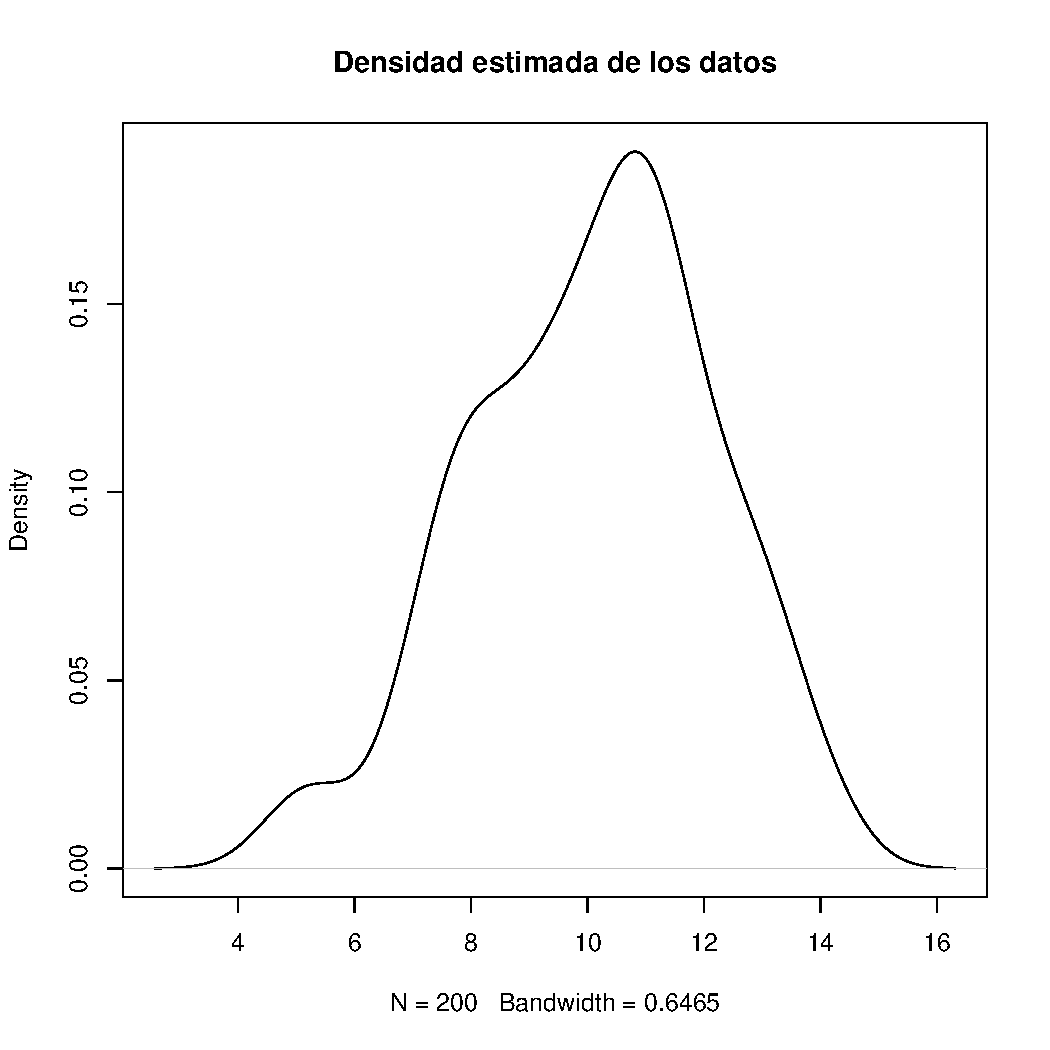
\includegraphics[width=\maxwidth]{figure/unnamed-chunk-16-2} 
\begin{kframe}\begin{alltt}
\hlcom{# R permite calcular la funci\textbackslash{}'on de distribuci\textbackslash{}'on acumulada te\textbackslash{}'orica con ecdf() }
\hlkwd{plot}\hlstd{(}\hlkwd{ecdf}\hlstd{(x.norm),}\hlkwc{main}\hlstd{=}\hlstr{"Función de distribución acumulada teórica"}\hlstd{)}
\end{alltt}
\end{kframe}
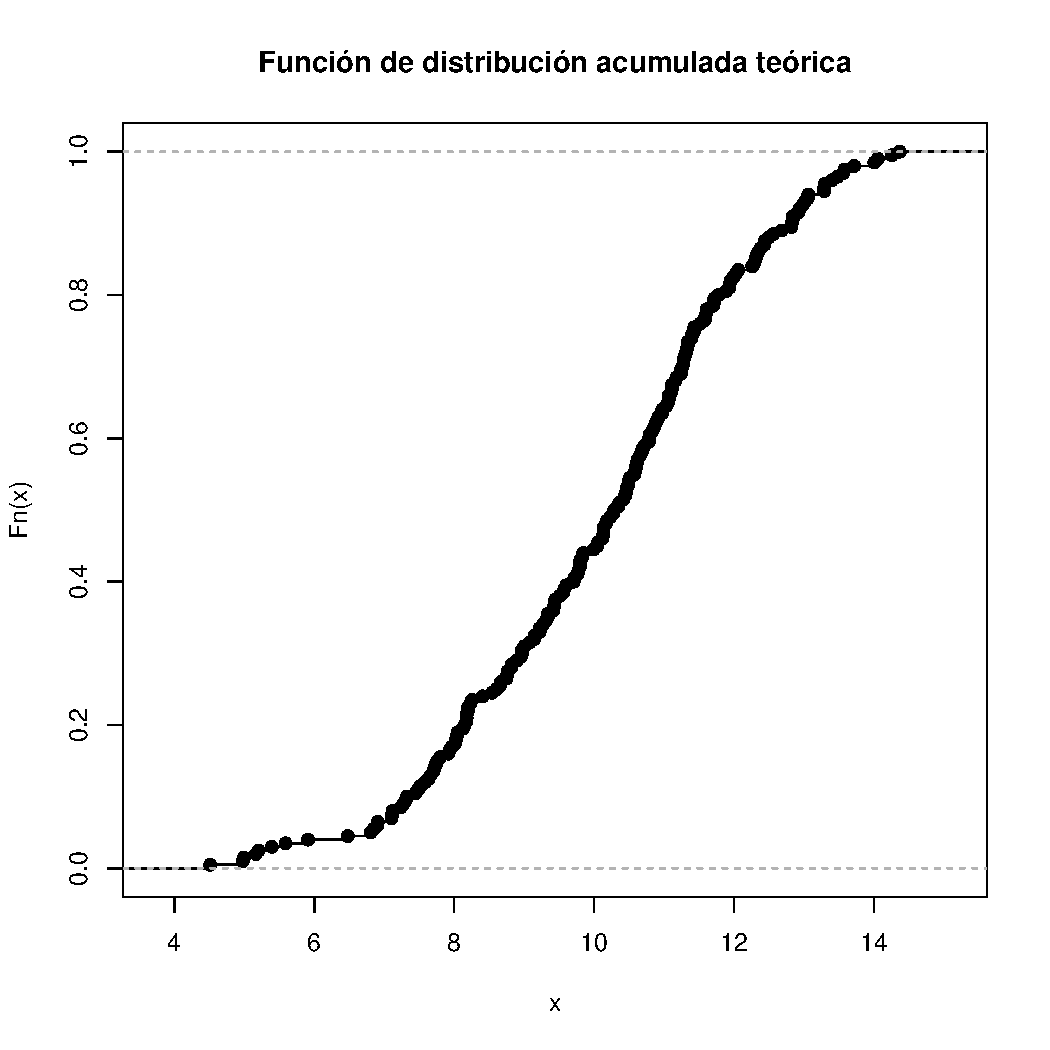
\includegraphics[width=\maxwidth]{figure/unnamed-chunk-16-3} 

\end{knitrout}

\begin{itemize}
  \item \textbf{Ejemplo 3:}
\end{itemize}
Generar 100 n\'umeros aleatorios de una distribuci\'on Normal con media 4.5 y desviaci\'on est\'andar 0.75.
\begin{knitrout}
\definecolor{shadecolor}{rgb}{0.969, 0.969, 0.969}\color{fgcolor}\begin{kframe}
\begin{alltt}
\hlcom{# Definir los par\textbackslash{}'ametros apropiados }
\hlstd{media} \hlkwb{<-} \hlnum{4.5}\hlstd{; desviacion} \hlkwb{<-} \hlnum{0.75}

\hlcom{# generar 100 n\textbackslash{}'umeros aleatorios de la distribuci\textbackslash{}'on }
\hlstd{x} \hlkwb{=} \hlkwd{rnorm}\hlstd{(}\hlnum{100}\hlstd{, media, desviacion); x}
\end{alltt}
\begin{verbatim}
##   [1] 4.685023 4.085347 4.690376 3.716264 3.538028 4.245896 4.293525
##   [8] 5.005417 6.363610 4.221063 3.748988 2.983803 4.364624 5.431396
##  [15] 5.469190 4.107875 4.119808 4.043912 3.405542 3.949332 3.828855
##  [22] 5.816811 4.922200 4.774044 4.708622 5.502216 3.998810 5.457184
##  [29] 5.450010 3.789861 4.658435 5.258724 4.371644 4.581935 5.365355
##  [36] 5.777487 2.846609 4.955483 4.981274 4.495799 5.188280 3.793359
##  [43] 3.649243 5.562281 4.093415 4.537764 3.140547 4.435097 3.845908
##  [50] 5.309575 4.703681 4.852680 3.921677 3.118858 4.686166 5.888000
##  [57] 2.917225 4.563399 4.727328 4.074747 4.468296 4.893315 4.260960
##  [64] 5.775534 3.290102 3.280047 4.348795 3.478990 4.848428 5.048595
##  [71] 3.997954 5.127976 4.873776 4.185929 4.733015 4.780149 5.106116
##  [78] 4.343931 4.324382 5.457152 2.985052 3.838946 4.374825 4.796517
##  [85] 4.332632 3.491315 3.624708 3.992557 3.403156 4.329689 4.838943
##  [92] 4.420180 3.375388 5.567997 5.907756 5.577851 5.023092 4.426826
##  [99] 4.743798 4.627503
\end{verbatim}
\begin{alltt}
\hlcom{# Histograma para la nuestra aleatoria de tama\textbackslash{}~no 100 }
\hlkwd{hist}\hlstd{(x,}\hlkwc{main}\hlstd{=}\hlkwd{expression}\hlstd{(}\hlkwd{paste}\hlstd{(}\hlstr{"X ~ N("}\hlstd{, mu,} \hlstr{" = 4.5, "}\hlstd{, sigma,} \hlstr{" = 0.75)"}\hlstd{)),}
\hlkwc{xlab}\hlstd{=}\hlstr{"X"}\hlstd{,} \hlkwc{ylab}\hlstd{=}\hlstr{"densidad de probabilidad"}\hlstd{,} \hlkwc{probability}\hlstd{=}\hlnum{TRUE}\hlstd{,} \hlkwc{col}\hlstd{=}\hlkwd{gray}\hlstd{(}\hlnum{0.9}\hlstd{))}

\hlcom{# Graficar la funci\textbackslash{}'on de densidad te\textbackslash{}'orica, usando la funci\textbackslash{}'on curve() }
\hlkwd{curve}\hlstd{(}\hlkwd{dnorm}\hlstd{(x, media, desviacion),} \hlkwc{col}\hlstd{=}\hlstr{"red"}\hlstd{,} \hlkwc{lwd}\hlstd{=}\hlnum{2}\hlstd{,} \hlkwc{add}\hlstd{=}\hlnum{TRUE}\hlstd{)}
\end{alltt}
\end{kframe}
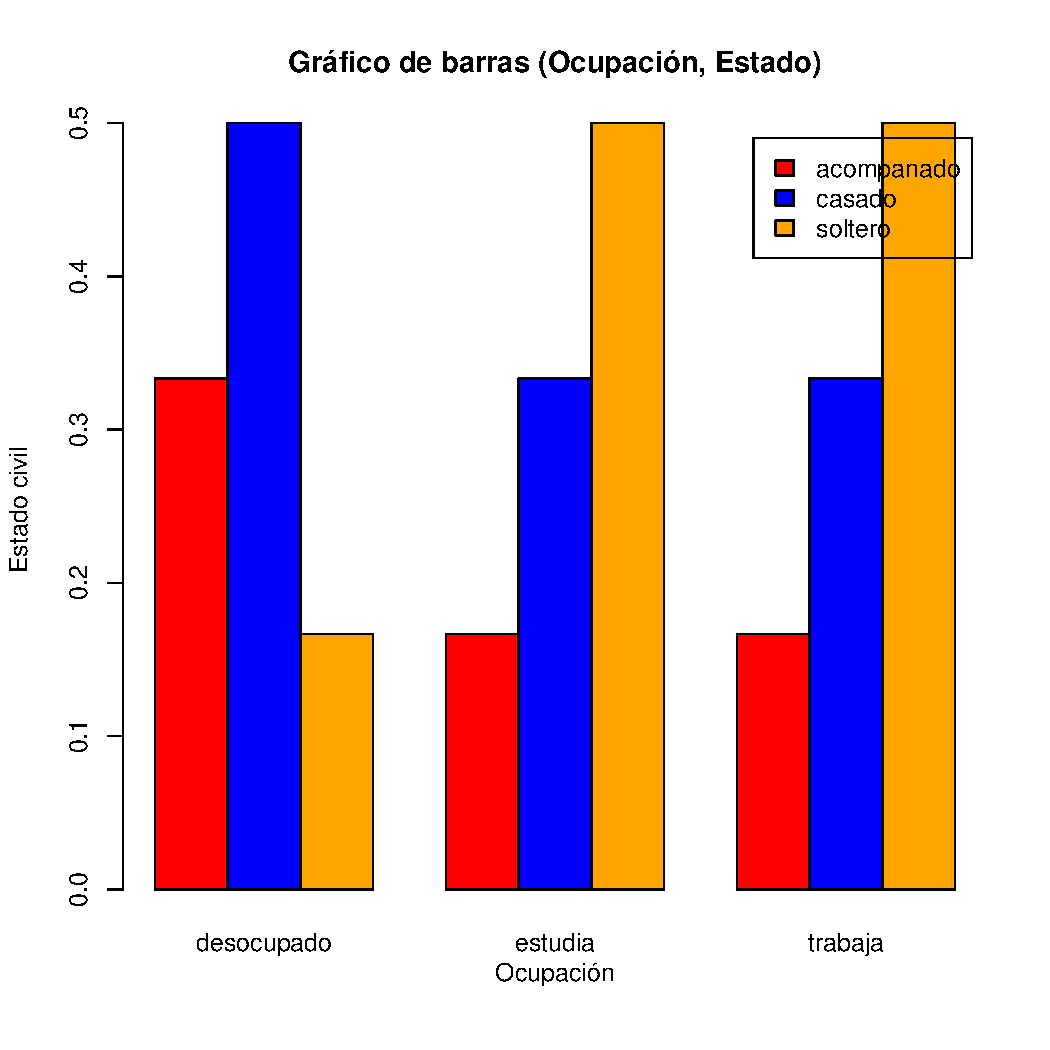
\includegraphics[width=\maxwidth]{figure/unnamed-chunk-17-1} 

\end{knitrout}

\begin{itemize}
  \item \textbf{Ejemplo 4:}
\end{itemize}
Generar n\'umeros aleatorios de una distribuci\'on exponencial. Por ejemplo, si la vida media de un bulbo de luz es 2500 horas, uno puede pensar que el tiempo de vida es aleatorio con una distribuci\'on exponencial que tiene media 2500. El \'unico par\'ametro es la raz\'on = 1/media.
\begin{knitrout}
\definecolor{shadecolor}{rgb}{0.969, 0.969, 0.969}\color{fgcolor}\begin{kframe}
\begin{alltt}
\hlcom{# Definir el par\textbackslash{}'ametro apropiado }
\hlstd{media} \hlkwb{<-} \hlnum{2500}\hlstd{; razon} \hlkwb{<-} \hlnum{1}\hlopt{/}\hlstd{media;n}\hlkwb{=}\hlnum{100}

\hlcom{# generar 100 números aleatorios de la distribuci\textbackslash{}'on }
\hlstd{x} \hlkwb{=} \hlkwd{rexp}\hlstd{(n, razon); x}
\end{alltt}
\begin{verbatim}
##   [1]  1497.05352  2525.29060  5840.21211  1615.22462  1235.99915
##   [6]  1639.14642  2325.65573  1006.30196  4043.57293   240.55050
##  [11]  2379.63817   902.40007  6424.37764    82.32148  1272.07182
##  [16]  6219.89923  1264.66282  2233.16240  3766.28769  1711.45686
##  [21]   245.22321  4045.29514   299.87246  2378.78900  2387.13219
##  [26]  3349.28066  1365.44929  1915.70584  1144.70006  5624.30359
##  [31]  7427.56721  3022.84775  2382.77466  5968.15114   119.00098
##  [36]   243.42030   558.75517  1920.82684  2966.77171  3632.56684
##  [41]  4580.18906  9928.03359   700.47084  3658.40637   510.15105
##  [46]  1152.04048   579.53950   296.50453  1926.53039  1508.98988
##  [51]  1420.28350  4982.12799  2941.88125   556.30561  3199.28647
##  [56]   825.67994   624.48165  1927.20463  2783.47374  5258.49014
##  [61]   716.79397   942.67333  2638.15169  1649.51976   749.34006
##  [66]  2221.83473 12281.61486   920.61243  1902.75934   976.64014
##  [71]  1381.90697  3352.22399  2490.22503  1354.78209  1554.19017
##  [76]  1012.72515  1755.05837  5745.37882  1138.64851  1708.48026
##  [81]  1065.43021  1308.05210  6920.78363  1333.33177  1435.59109
##  [86]  1334.11109   910.88817  2546.68384   439.87444  2670.88157
##  [91]  2279.90290  1376.39155  3669.47212  1561.55536    74.15215
##  [96]   412.24977    26.54866  1090.88679  3123.18052  1047.65997
\end{verbatim}
\begin{alltt}
\hlcom{# Histograma para la nuestra aleatoria de tama\textbackslash{}~no 100 }
\hlkwd{hist}\hlstd{(x,} \hlkwc{main}\hlstd{=}\hlstr{"X ~ Exponencial( media = 2500 )"}\hlstd{,} \hlkwc{xlab}\hlstd{=}\hlstr{"X"}\hlstd{,}
     \hlkwc{ylab}\hlstd{=}\hlstr{"densidad de probabilidad"}\hlstd{,} \hlkwc{probability}\hlstd{=}\hlnum{TRUE}\hlstd{,} \hlkwc{col}\hlstd{=}\hlstr{"green"}\hlstd{)}

\hlcom{# Graficar la funci\textbackslash{}'on de densidad, usando la funci\textbackslash{}'on curve() }
\hlkwd{curve}\hlstd{(}\hlkwd{dexp}\hlstd{(x, razon),} \hlkwc{col}\hlstd{=}\hlstr{"blue"}\hlstd{,} \hlkwc{lwd}\hlstd{=}\hlnum{2}\hlstd{,} \hlkwc{add}\hlstd{=}\hlnum{TRUE}\hlstd{)}
\end{alltt}
\end{kframe}
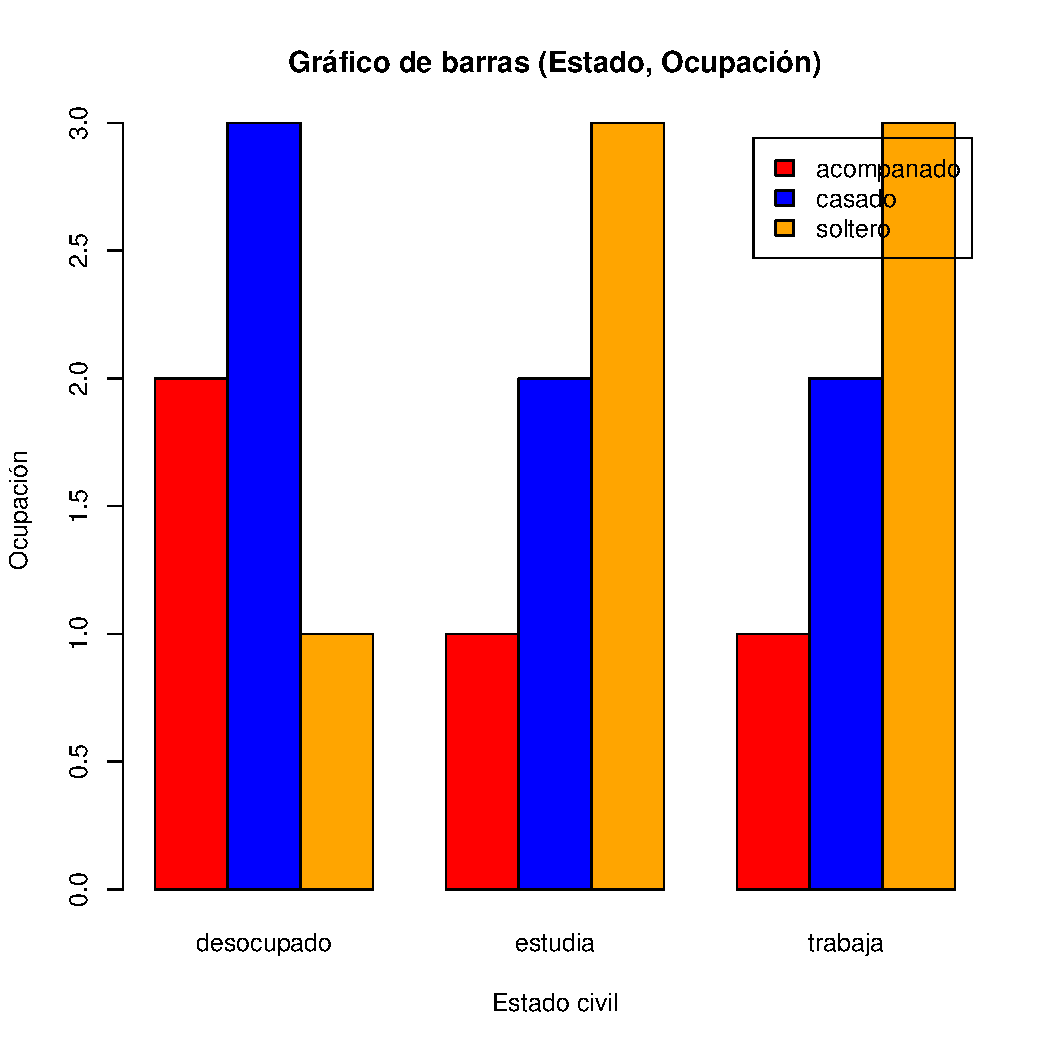
\includegraphics[width=\maxwidth]{figure/unnamed-chunk-18-1} 

\end{knitrout}

\newpage

\begin{center}
\textbf{4. FUNCIONES DE DISTRIBUCI\'ON Y SU INVERSA (LOS CUANTILES).}
\end{center}

En R, las funciones a las que se les antepone una "p" permiten contestar cu\'al es la probabilidad de que una variable aleatoria X sea menor o igual que x, esto es F(x)=P[X$<$=x]. Las funciones a las que se les antepone una "q" son lo inverso de esto, ellas permiten conocer qu\'e valor de una variable aleatoria X corresponde a una probabilidad p dada. Esto es el cuantil Xq o punto en el que los datos son partidos, P[X$<$=x_q]=p.\\

\begin{itemize}
  \item \textbf{Ejemplo 1:}
\end{itemize}
Para una Variable aleatoria X con distribuci\'on normal de media 1 y desviaci\'on 
est\'andar 1, \¿cu\'al es la probabilidad de que sea menor que 0.7?
\begin{knitrout}
\definecolor{shadecolor}{rgb}{0.969, 0.969, 0.969}\color{fgcolor}\begin{kframe}
\begin{alltt}
\hlstd{x} \hlkwb{<-} \hlnum{0.7}
\hlstd{p} \hlkwb{<-} \hlkwd{pnorm}\hlstd{(x,} \hlkwc{mean}\hlstd{=}\hlnum{1}\hlstd{,} \hlkwc{sd}\hlstd{=}\hlnum{1}\hlstd{,} \hlkwc{lower.tail} \hlstd{=} \hlnum{TRUE}\hlstd{); p}
\end{alltt}
\begin{verbatim}
## [1] 0.3820886
\end{verbatim}
\end{kframe}
\end{knitrout}
\textbf{Observaci\'on:} lower.tail=TRUE es el valor por defecto, para indicar las probabilidades son P[X$<$=x], en otro caso ser\'a P[X$>$x].\\

\begin{itemize}
  \item \textbf{Ejemplo 2:}
\end{itemize}
Para una variable aleatoria con distribuci\'on normal est\'andar, encontrar 
P[Z$<$=0.7] y P[Z$>$0.7]. 
\begin{knitrout}
\definecolor{shadecolor}{rgb}{0.969, 0.969, 0.969}\color{fgcolor}\begin{kframe}
\begin{alltt}
\hlstd{z} \hlkwb{<-} \hlnum{0.7}
\hlstd{p1} \hlkwb{<-} \hlkwd{pnorm}\hlstd{(z,} \hlkwc{mean}\hlstd{=}\hlnum{0}\hlstd{,} \hlkwc{sd}\hlstd{=}\hlnum{1}\hlstd{); p1}
\end{alltt}
\begin{verbatim}
## [1] 0.7580363
\end{verbatim}
\begin{alltt}
\hlstd{p2} \hlkwb{<-} \hlkwd{pnorm}\hlstd{(z,} \hlkwc{mean}\hlstd{=}\hlnum{0}\hlstd{,} \hlkwc{sd}\hlstd{=}\hlnum{1}\hlstd{,} \hlkwc{lower.tail}\hlstd{=}\hlnum{FALSE}\hlstd{); p2}
\end{alltt}
\begin{verbatim}
## [1] 0.2419637
\end{verbatim}
\end{kframe}
\end{knitrout}
\textbf{Observaci\'on:} ya que P[Z$>$0.7]=1-[Z$<$=0.7], obtenemos el mismo resultado con
\begin{knitrout}
\definecolor{shadecolor}{rgb}{0.969, 0.969, 0.969}\color{fgcolor}\begin{kframe}
\begin{alltt}
\hlstd{p3} \hlkwb{<-} \hlnum{1}\hlopt{-}\hlkwd{pnorm}\hlstd{(z,} \hlkwc{mean}\hlstd{=}\hlnum{0}\hlstd{,} \hlkwc{sd}\hlstd{=}\hlnum{1}\hlstd{);p3}
\end{alltt}
\begin{verbatim}
## [1] 0.2419637
\end{verbatim}
\end{kframe}
\end{knitrout}

\begin{itemize}
  \item \textbf{Ejemplo 3:}
\end{itemize}
\¿Qu\'e valor de una variable aleatoria con distribuci\'on normal est\'andar, tiene 75\% 
del \'area a la izquierda?. 
\begin{knitrout}
\definecolor{shadecolor}{rgb}{0.969, 0.969, 0.969}\color{fgcolor}\begin{kframe}
\begin{alltt}
\hlstd{p} \hlkwb{<-} \hlnum{0.75}
\hlstd{z} \hlkwb{<-} \hlkwd{qnorm}\hlstd{(p,} \hlkwc{mean}\hlstd{=}\hlnum{0}\hlstd{,} \hlkwc{sd}\hlstd{=}\hlnum{1}\hlstd{,} \hlkwc{lower.tail} \hlstd{=} \hlnum{TRUE}\hlstd{); z}
\end{alltt}
\begin{verbatim}
## [1] 0.6744898
\end{verbatim}
\end{kframe}
\end{knitrout}
\textbf{Observaci\'on:} note que el valor de z que resuelve P[Z$<$=z]=0.75 es el tercer cuartil (Q3), esto es z=0.6744898.

\begin{itemize}
  \item \textbf{Ejemplo 4:}
\end{itemize}
\¿Cu\'al es la probabilidad a la derecha de 18.55 para una Variable aleatoria X con 
distribuci\'on Chi-cuadrado de 12 grados de libertad?
\begin{knitrout}
\definecolor{shadecolor}{rgb}{0.969, 0.969, 0.969}\color{fgcolor}\begin{kframe}
\begin{alltt}
\hlstd{x} \hlkwb{<-} \hlnum{18.55}\hlstd{; gl} \hlkwb{<-} \hlnum{12}
\hlstd{p} \hlkwb{<-} \hlkwd{pchisq}\hlstd{(x, gl,} \hlkwc{lower.tail} \hlstd{=} \hlnum{FALSE}\hlstd{); p}
\end{alltt}
\begin{verbatim}
## [1] 0.09998251
\end{verbatim}
\end{kframe}
\end{knitrout}











\end{document}
